\documentclass{ansarticle-preprint}
%\usepackage{ucs}
\usepackage[utf8]{inputenc}
\usepackage{amsmath}
%\usepackage{cite}
\usepackage{anslistings}
\usepackage{multicol}
\usepackage{pdfsync}

\usepackage{pgfplots}
\usepackage{pgfplotstable}

\usepackage{fontenc}
\usepackage{graphicx}
\usepackage{xspace}

\usepackage{siunitx}

\usepackage{floatflt}

\usepackage{multirow}

%\renewcommand{\baselinestretch}{2.0}

\usepackage[normalem]{ulem}

\usepackage{todonotes}

\pgfplotsset{compat=1.9}
\definecolor{gnuplot@lightblue}{RGB}{87,181,232}
\definecolor{gnuplot@green}{RGB}{0,158,115}
\definecolor{gnuplot@purple}{RGB}{148,0,212}

\newcommand{\specialword}[1]{\texttt{#1}}
\newcommand{\dealii}{{\specialword{deal.II}}\xspace}
\newcommand{\pfrst}{{\specialword{p4est}}\xspace}
\newcommand{\trilinos}{{\specialword{Trilinos}}\xspace}
\newcommand{\aspect}{\specialword{Aspect}\xspace}
\newcommand{\petsc}{\specialword{PETSc}\xspace}
\newcommand{\cmake}{{\specialword{CMake}}\xspace}
\newcommand{\autoconf}{{\specialword{autoconf}}\xspace}


\usetikzlibrary{shapes.misc}
\tikzset{cross/.style={cross out, draw=black, minimum size=2*(#1-\pgflinewidth), inner sep=0pt, outer sep=0pt},
%default radius will be 1pt.
cross/.default={2pt}}

%
% Author list -- please add yourself in both places below (in
%                alphabetical order) if you think that your
%                contributions to the last release warrant this
%

\hypersetup{
  pdfauthor={
     Daniel Arndt,
     Wolfgang Bangerth,
     %Bruno Blais,
     %Thomas C. Clevenger,
    Marc Fehling,
    %Alexander V. Grayver,
    Timo Heister,
    Luca Heltai,
    Martin Kronbichler,
    Matthias Maier,
    Peter Munch,
    Jean-Paul Pelteret,
    %Reza Rastak,
    %Ignacio Thomas,
    Bruno Turcksin,
    %Zhuoran Wang,
    David Wells
  },
  pdftitle={The deal.II Library, Version 9.3, 2021},
}

\title{The \dealii{} Library, Version 9.3}

 \author[*1]{Daniel Arndt}
 \affil[1]{Computational Engineering and Energy Sciences Group,
   Computational Sciences and Engineering Division,
   Oak Ridge National Laboratory, 1 Bethel Valley Rd.,
   TN 37831, USA.
   \texttt{arndtd/turcksinbr@ornl.gov}}

 \author[2]{Wolfgang~Bangerth}
 \affil[2]{Department of Mathematics and Department of Geosciences, Colorado State University, Fort
   Collins, CO 80523-1874, USA.
   \texttt{bangerth@colostate.edu}}


%\author[3]{Bruno Blais}
%\affil[3]{Research Unit for Industrial Flows Processes (URPEI), Department of Chemical Engineering,
%          Polytechnique Montréal,
%          PO Box 6079, Stn Centre-Ville, Montréal, Québec, Canada, H3C 3A7.
%          {\texttt{bruno.blais@polymtl.ca}}}

% \author[4]{Thomas~C.~Clevenger}
% \affil[4]{School of Mathematical and Statistical Sciences,
%   Clemson University,
%   Clemson, SC, 29634, USA
%   {\texttt{tcleven/heister@clemson.edu}}}
%
% \author[4]{Denis~Davydov}
% \affil[4]{Chair of Applied Mechanics,
%   Friedrich-Alexander-Universit\"{a}t Erlangen-N\"{u}rnberg,
%   Egerlandstr.\ 5,
%   91058 Erlangen, Germany.
%   {\texttt{\{denis.davydov,jean-paul.pelteret\}@fau.de}}}
%
\author[5]{Marc~Fehling}
\affil[5]{Institute for Advanced Simulation,
  Forschungszentrum J\"{u}lich GmbH,
  52425 J\"{u}lich, Germany.
  {\texttt{m.fehling@fz-juelich.de}}}
%
% \author[6]{Daniel Garcia-Sanchez}
% \affil[6]{Sorbonne Universit\'es, UPMC Univ.\ Paris 06, CNRS-UMR 7588,
%   Institut des NanoSciences de Paris, F-75005, Paris, France
%   {\texttt{daniel.garcia-sanchez@insp.upmc.fr}}}
%
% \author[2]{Graham Harper}
%

%\author[6]{Alexander~V.~Grayver}
%\affil[6]{Institute of Geophysics,
%  ETH Zurich,
%  Sonneggstrasse 5, 8092 Z\"{u}rich, Switzerland.
%  {\texttt{agrayver@ethz.ch}}}

\author[4]{Timo~Heister}

\author[7]{Luca~Heltai}
\affil[7]{SISSA,
   International School for Advanced Studies,
   Via Bonomea 265,
   34136, Trieste, Italy.
   {\texttt{luca.heltai@sissa.it}}}

 \author[8]{Martin~Kronbichler}
 \affil[8]{Institute for Computational Mechanics,
   Technical University of Munich,
   Boltzmannstr.~15, 85748 Garching, Germany.
   {\texttt{kronbichler/munch@lnm.mw.tum.de}}}

\author[9]{Matthias~Maier}
\affil[9]{Department of Mathematics,
  Texas A\&M University,
  3368 TAMU,
  College Station, TX 77845, USA.
  {\texttt{maier@math.tamu.edu}}}

\author[8,10]{Peter Munch}
 \affil[10]{Institute of Materials Research, Materials Mechanics,
 Helmholtz-Zentrum Geesthacht,
 Max-Planck-Str. 1, 21502 Geesthacht, Germany.
   {\texttt{peter.muench@hzg.de}}}


\author[11]{Jean-Paul~Pelteret}
\affil[11]{Independent researcher.
{\texttt{jppelteret@gmail.com}}}

% \author[12]{Reza Rastak}
% \affil[12]{Department of Civil and Environmental Engineering,
%   Stanford University,
%   Stanford, CA 94305, USA.
%   {\texttt{rastak@stanford.edu}}}

% \author[**13]{Ignacio Tomas}
% \affil[13]{Sandia National Laboratories, Org 1442,
% P.O. Box 5800, MS 1320, Albuquerque, NM, 87185-1320,
%   \texttt{itomas@sandia.gov}}

\author[*1]{Bruno~Turcksin}
%

%\author[14]{Zhuoran Wang}
%\affil[14]{Department of Mathematics, Colorado State University, Fort Collins,
%          CO 80523-1874, USA.
%{\texttt{zhrwang@math.colostate.edu}}}

\author[15]{David Wells}
\affil[15]{Department of Mathematics, University of North Carolina,
  Chapel Hill, NC 27516, USA.
  {\texttt{drwells@email.unc.edu}}}

\renewcommand{\labelitemi}{--}


\begin{document}
\maketitle

\footnotetext{%
  $^\ast$ This manuscript has been authored by UT-Battelle, LLC under Contract No.
  DE-AC05-00OR22725 with the U.S. Department of Energy.
  %The United States
  %Government retains and the publisher, by accepting the article for
  %publication, acknowledges that the United States Government retains a
  %non-exclusive, paid-up, irrevocable, worldwide license to publish or reproduce
  %the published form of this manuscript, or allow others to do so, for United
  %States Government purposes. The Department of Energy will provide public
  %access to these results of federally sponsored research in accordance with the
  %DOE Public Access Plan (http://energy.gov/downloads/doe-public-access-plan).
}

\footnotetext{%
  $^{**}$ Sandia National Laboratories is a multimission laboratory managed and
  operated by National Technology \& Engineering Solutions of Sandia, LLC, a
  wholly owned subsidiary of Honeywell International Inc., for the U.S.
  Department of Energy's National Nuclear Security Administration under contract
  DE-NA0003525. This document describes objective technical results and analysis.
  Any subjective views or opinions that might be expressed in the paper do not
  necessarily represent the views of the U.S. Department of Energy or the United
  States Government.}

\begin{abstract}
  This paper provides an overview of the new features of the finite element
  library \dealii, version 9.3.
\end{abstract}



%%%%%%%%%%%%%%%%%%%%%%%%%%%%%%%%%%%%%%%%%%%%%%%%%%%%%%%%%%%%%%%%%%%%%%%%%%%%%%%%
%%%%%%%%%%%%%%%%%%%%%%%%%%%%%%%%%%%%%%%%%%%%%%%%%%%%%%%%%%%%%%%%%%%%%%%%%%%%%%%%
%%%%%%%%%%%%%%%%%%%%%%%%%%%%%%%%%%%%%%%%%%%%%%%%%%%%%%%%%%%%%%%%%%%%%%%%%%%%%%%%
\section{Overview}

\dealii{} version 9.3.0 was released May ??, 2021.
This paper provides an
overview of the new features of this release and serves as a citable
reference for the \dealii{} software library version 9.3. \dealii{} is an
object-oriented finite element library used around the world in the
development of finite element solvers. It is available for free under the
GNU Lesser General Public License (LGPL). Downloads are available at
\url{https://www.dealii.org/} and \url{https://github.com/dealii/dealii}.

The major changes of this release are:
%
\begin{itemize}
  \item TODO.
\end{itemize}
%
These major changes are discussed in detail in Section~\ref{sec:major}. There
are a number of other noteworthy changes in the current \dealii{} release
that we briefly outline in the remainder of this section:
%
\begin{itemize}
  \item globally unique cell IDs: TODO
\end{itemize}
%
The changelog lists more than 240 other
features and bugfixes.




%%%%%%%%%%%%%%%%%%%%%%%%%%%%%%%%%%%%%%%%%%%%%%%%%%%%%%%%%%%%%%%%%%%%%%%%%%%%%%%%
%%%%%%%%%%%%%%%%%%%%%%%%%%%%%%%%%%%%%%%%%%%%%%%%%%%%%%%%%%%%%%%%%%%%%%%%%%%%%%%%
%%%%%%%%%%%%%%%%%%%%%%%%%%%%%%%%%%%%%%%%%%%%%%%%%%%%%%%%%%%%%%%%%%%%%%%%%%%%%%%%
\section{Major changes to the library}
\label{sec:major}

This release of \dealii{} contains a number of large and significant changes
that will be discussed in this section.
It of course also contains a
vast number of smaller changes and added functionality; the details of these
can be found
\href{https://dealii.org/developer/doxygen/deal.II/changes_between_9_2_0_and_9_3_0.html}
{in the file that lists all changes for this release}; see \cite{changes93}.

%\newpage

%%%%%%%%%%%%%%%%%%%%%%%%%%%%%%%%%%%%%%%%%%%%%%%%%%%%%%%%%%%%%%%%%%%%%%%%%%%%%%%%
\subsection{Simplex and mixed mesh support}
\label{subsec:simplex}

\begin{figure}[!h]

\centering


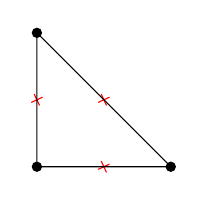
\begin{tikzpicture}[scale=1.7]

\coordinate (0) at (0,0);
\coordinate (1) at (1,0);
\coordinate (2) at (0,1);

\coordinate (3) at (0,0.5);
\coordinate (4) at (0.5,0.5);
\coordinate (5) at (0.5,0);

\foreach \i in {0,1, 2}
    \fill (\i) circle (1.1pt) node [below] {};

\foreach \i in {3,4,5}
    \draw (\i) node[cross, draw=red, rotate=-20] {};


\draw (0) --(1) -- (2) -- (0);

\end{tikzpicture}
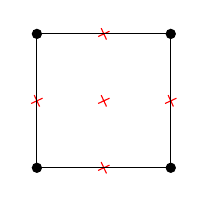
\begin{tikzpicture}[scale=1.7]

\coordinate (0) at (0,0);
\coordinate (1) at (1,0);
\coordinate (2) at (1,1);
\coordinate (3) at (0,1);


\coordinate (4) at (0.5,0,0);
\coordinate (5) at (1.0,0.5);
\coordinate (6) at (0.0,0.5);
\coordinate (7) at (0.5,1.0);
\coordinate (8) at (0.5,0.5);

\foreach \i in {0,1, 2, 3}
    \fill (\i) circle (1.1pt) node [below] {};


\foreach \i in {4,5,6,7,8}
    \draw (\i) node[cross, draw=red, rotate=-20] {};


\draw (0) --(1) -- (2) -- (3) -- (0);

\end{tikzpicture}
\qquad\qquad
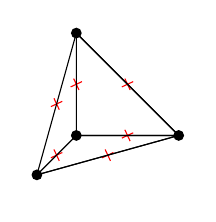
\begin{tikzpicture}[scale=1.3]

\coordinate (0) at (0,0,0);
\coordinate (1) at (1,0,0);
\coordinate (2) at (0,1,0);
\coordinate (3) at (0,0,1);

\coordinate (4) at (0.5,0,0);
\coordinate (5) at (0,0.5,0);
\coordinate (6) at (0,0,0.5);
\coordinate (7) at (0.5,0.5,0.0);
\coordinate (8) at (0.5,0.0,0.5);
\coordinate (9) at (0.0,0.5,0.5);


\foreach \i in {0,1,2,3}
    \fill (\i) circle (1.5pt) node [below] {};


\foreach \i in {4,5,6,7,8,9}
    \draw (\i) node[cross, draw=red, rotate=-20] {};


\draw (0) -- (1) -- (2) -- (0);
\draw (0) -- (1) -- (3) -- (0);
\draw (1) -- (2) -- (3) -- (1);

\end{tikzpicture}
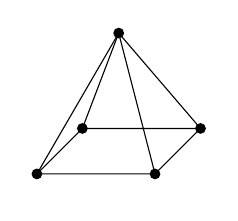
\begin{tikzpicture}[scale=1.5]

\coordinate (0) at (0.0, 0.0, 0.0);
\coordinate (1) at (0.0, 0.0, 1.0);
\coordinate (2) at (1.0, 0.0, 0.0);
\coordinate (3) at (1.0, 0.0, 1.0);
\coordinate (4) at (0.5, 1.0, 0.5);

\coordinate  (5) at (0.5, 0.0, 0.0);
\coordinate  (6) at (0.0, 0.0, 0.5);
\coordinate  (7) at (0.5, 0.0, 1.0);
\coordinate  (8) at (1.0, 0.0, 0.5);

\coordinate  (9) at (0.25,0.5,0.25);
\coordinate (10) at (0.25,0.5,0.75);
\coordinate (11) at (0.75,0.5,0.25);
\coordinate (12) at (0.75,0.5,0.75);


\coordinate (13) at (0.5, 0.0, 0.5);

\foreach \i in {0,1,2,3,4}
    \fill (\i) circle (1.3pt) node [below] {};


%\foreach \i in {5, 6, 7, 8, 9, 10, 11, 12, 13}
%    \draw (\i) node[cross] {};


\draw (0) -- (1) -- (3) -- (2) -- (0);
\draw (1) -- (4) -- (3);
\draw (0) -- (4) -- (2);

\end{tikzpicture}
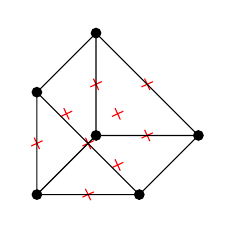
\begin{tikzpicture}[scale=1.3]

\coordinate (0) at (0,0,1.5);
\coordinate (1) at (1,0,1.5);
\coordinate (2) at (0.0,1.0,1.5);

\coordinate (3) at (0,0,0);
\coordinate (4) at (1,0,0);
\coordinate (5) at (0.0,1.0,0);



\coordinate  (6) at (0.5, 0.0, 0.0);
\coordinate  (7) at (0.0, 0.5, 0.0);
\coordinate  (8) at (0.5, 0.5, 0.0);

\coordinate   (9) at (0.5, 0.0, 0.75);
\coordinate  (10) at (0.0, 0.5, 0.75);
\coordinate  (11) at (0.5, 0.5, 0.75);

\coordinate  (12) at (0.5, 0.0, 1.5);
\coordinate  (13) at (0.0, 0.5, 1.5);
\coordinate  (14) at (0.5, 0.5, 1.5);

\foreach \i in {0,1,2,3,4,5}
    \fill (\i) circle (1.5pt) node [below] {};

\foreach \i in {6,7,8,9,10,11,12,13,14}
    \draw (\i) node[cross, draw=red, rotate=-20] {};


\draw (0) -- (1) -- (2) -- (0);
\draw (3) -- (4) -- (5) -- (3);
\draw (0) -- (3);
\draw (1) -- (4);
\draw (2) -- (5);

\end{tikzpicture}
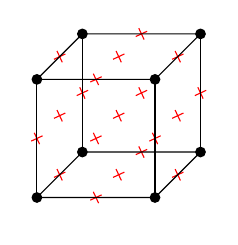
\begin{tikzpicture}[scale=1.5]

\coordinate (0) at (0,0,1);
\coordinate (1) at (1,0,1);
\coordinate (2) at (0,0,0);
\coordinate (3) at (1,0,0);

\coordinate (4) at (0,1,1);
\coordinate (5) at (1,1,1);
\coordinate (6) at (0,1,0);
\coordinate (7) at (1,1,0);

\coordinate  (8) at (0,0,0.5);
\coordinate  (9) at (1,0,0.5);
\coordinate (10) at (0.5,0,1);
\coordinate (11) at (0.5,0,0);
\coordinate (12) at (0.5,0,0.5);

\coordinate (13) at (0,1,0.5);
\coordinate (14) at (1,1,0.5);
\coordinate (15) at (0.5,1,1);
\coordinate (16) at (0.5,1,0);
\coordinate (17) at (0.5,1,0.5);


\coordinate (18) at (0,0.5,1);
\coordinate (19) at (1,0.5,1);
\coordinate (20) at (0,0.5,0);
\coordinate (21) at (1,0.5,0);
\coordinate (22) at (0,0.5,0.5);
\coordinate (23) at (1,0.5,0.5);
\coordinate (24) at (0.5,0.5,1);
\coordinate (25) at (0.5,0.5,0);
\coordinate (26) at (0.5,0.5,0.5);



\foreach \i in {0,1,2,3,4,5,6,7}
    \fill (\i) circle (1.3pt) node [below] {};

\foreach \i in {8,9,10,11,12,13,14,15,16,17,18,19,20,21,22,23,24,25,26}
    \draw (\i) node[cross, draw=red, rotate=-20] {};


\draw (0) -- (1) -- (3) -- (2) -- (0);
\draw (4) -- (5) -- (7) -- (6) -- (4);
\draw (0) -- (4);
\draw (1) -- (5);
\draw (2) -- (6);
\draw (3) -- (7);

\end{tikzpicture}

\caption{All reference cells in 2D (triangle, quadrilateral) and 3D (tetrahedron, pyramid, wedge, hexahedron) with the support points indicated both for linear ($\bullet$) and quadratic ($\times$) shape functions.}

\end{figure}

\begin{table}[!h]
  \caption{\it List of new scalar \texttt{FiniteElement} classes for the new
  reference-cell types. Vectorial elements can be constructed based on these classes
  via \texttt{FE\_Systems}.}\label{tab:simplex:fe}
  \centering
  \begin{tabular}{cccc}
    \toprule
    \textbf{reference cell} & \textbf{finite element} & \textbf{dimension} & \textbf{degree}\\
    \midrule
    \multirow{2}{*}{simplex (line, triangle, tetrahedron)} & FE\_SimplexP, FE\_SimplexDGP  & 1--3 & 1--2 \\
                                          & FE\_SimplexP\_Bubbles  & 1--3 & 1--2 \\
    pyramid & FE\_PyramidP, FE\_PyramidDGP  & 3 & 1 \\
    wedge & FE\_WedgeP, FE\_WedgeDGP  & 3 & 1--2 \\
    \bottomrule
  \end{tabular}
\end{table}

The current release of \dealii adds support for simplex meshes (consisting of triangles in 2D; tetrahedra in 3D) and mixed meshes (consisting of triangles and/or
quadrilaterals in 2D; tetrahedra, pyramids, wedges, and/or hexahedra in 3D).
Many freely available mesh-generation tools produce such kind of meshes; while users of \dealii used to have to pre-process such meshes and convert them to pure hex meshes, they
can now directly work with them.

\subsubsection{Refactoring of internal data structures}

To enable simplex and mixed mesh support, we performed a major refactoring of the internal data structures of \dealii. In particular, the \texttt{Triangulation} class and
the \texttt{DoFHandler} class have undergone large changes.

The template parameters of the internal data structures of \texttt{Triangulation}
have been removed and the type of each cell and of each face (only in 3D) is stored. The function
\texttt{Triangulation::create\_\allowbreak triangulation()}, which converts a given list of
cells and vertices to the internal data structures, has been rewritten
inspired by \citep{logg09} and a speed-up of up to 5 has been reached. Minor adjustments
have been made to \texttt{parallel::shared::Triangulation} and \texttt{parallel::\allowbreak fullydistributed::\allowbreak Triangulation} such that
the new mesh types can be processed also in parallel.

The internal data structures of \texttt{DoFHandler} used to be hard-coded for pure
hypercube meshes, while the \texttt{hp::DoFHandler} used to be built around
CRS-like data structures. Due to the need of CRS data structures in the
\texttt{DoFHandler} in the context of more general meshes, we have merged
\texttt{hp::DoFHandler} into the \texttt{DoFHandler}. The class \texttt{hp::DoFHandler}, which is now a dummy derivation of \texttt{DoFHandler}, currently only exists for compatibility reasons. For
more details see Subsection~\ref{TODO}.

\subsubsection{Generating meshes}

The most obvious way to generate a simplex or a mixed mesh is to read the mesh from a file
generated by an external mesh generator. Currently, we support the
file formats \texttt{VTK}, \texttt{MSH}, \texttt{EXODUS II}.

Alternatively, one can create a pure hypercube mesh with the known functions
in the \texttt{GridGenerator} namespace and convert the obtained mesh to a
pure simplex mesh with the function
\texttt{convert\_\allowbreak hypercube\_\allowbreak to\_\allowbreak simplex\_\allowbreak mesh()} from the \texttt{GridGenerator} namespace.

\subsubsection{Simplex mesh}

After having created a triangulation, one can proceed as usual in the case of
a pure simplex mesh by selecting an appropriate finite element, mapping, and
quadrature class:

\begin{c++}
FE_SimplexP<dim, spacedim> fe(degree);
MappingFE<dim, spacedim> mapping(FE_SimplexP<dim, spacedim>(1));
QGaussSimplex<dim> quad(degree + 1);

DoFHandler<dim> dof_handler(tria);
dof_handler.distribute_dofs(fe);

FEValues<dim, spacedim> fe_values(mapping, fe, quad, flags);
\end{c++}
The  list of currently supported finite-element classes is provided in Table~\ref{tab:simplex:fe}. Currently,
only linear iso-parametric mapping (\texttt{MappingFE} and \texttt{MappingFEFields}) is available. For quadrature, the classes \texttt{QGaussSimplex}, \texttt{QWitherdenVincentSimplex},
\texttt{QGaussPyamid}, and \texttt{QGaussWedge} are
available.

\subsubsection{Mixed mesh}
For mixed meshes, concepts known from the $hp$-context have been applied:
 different finite-element classes are assigned to different cell types. In the
case of a 2D mixed mesh, which can only consists of triangles and
quadrilaterals, the finite element defined on a triangle (e.g., \texttt{FE\_SimplexP})
and on a quadrilateral (e.g., \texttt{FE\_Q}) can be collected in a \texttt{hp::FECollection}:

\begin{c++}
hp::FECollection<dim, spacedim> fe
  {FE_SimplexP<dim, spacedim>(degree), FE_Q<dim, spacedim>(degree)};
\end{c++}

Similarly, \texttt{hp::QCollection} and \texttt{hp::MappingCollection} can be used
to construct appropriate collections. Furthermore, the right active finite-element index, which points to the right
finite element of that cell, has to be assigned to each cell:

\begin{c++}
DoFHandler<dim> dof_handler(tria);

for (const auto &cell : dof_handler.active_cell_iterators())
  switch(cell->reference_cell_type())
    {
      case ReferenceCell::Type::Tri:  cell->set_active_fe_index(0); break;
      case ReferenceCell::Type::Quad: cell->set_active_fe_index(1); break;
      // 3D (Tet, Pyramid, Wedge, Hex) not shown
      default: Assert(false, ExcNotImplemented());
    }

dof_handler.distribute_dofs(fe);
\end{c++}

\subsubsection{Practical implications}

The introduction of simplex and mixed meshes leads to some implications
for the user if these features should be used. For instance, each cell might have a different type with
different number of vertices, lines, and faces so that these quantities can not be
compile-time constants anymore. This information used to be queried from
the \texttt{GeometryInfo} class. To avoid using this class, we have extended
relevant classes, e.g., \texttt{TriaAccessor} or \texttt{TriaCellAccessor},
with useful new functions like \texttt{n\_vertices()}, \texttt{n\_lines()}, or
\texttt{n\_faces()} so that users can simply write:
\begin{c++}
for(const auto & cell : tria.active_cell_iterators())
  for(unsigned int f = 0; f < cell->n_faces(); ++f)
    (void) cell->face(f);
\end{c++}
Alternatively, one can use an iterator-based approach to loop over all faces
of a cell, introduced in the last release. The relevant functions have been adjusted to be able to deal with
various number of faces.
\begin{c++}
for(const auto & cell : tria.active_cell_iterators())
  for(const auto & face : cell->face_iterators())
    (void) face;
\end{c++}
Furthermore, the number of degrees of freedom might differ between cells so that
local data storage units needed for assembly might need to be resized for each
cell as it is already good practice in the $hp$-context:
\begin{c++}
std::vector<double> local_rhs;
for(const auto & cell : tria.active_cell_iterators())
 {
   hp_fe_values.reinit(cell);
   local_rhs.resize(hp_fe_values.get_present_fe_values().n_dofs_per_cell());
 }
\end{c++}


What is true for cells is also true for faces in 3D: faces can be either triangles
or quadrilaterals. This is the case even if no mixed mesh is used. As a consequence, some functions, e.g. \texttt{FiniteElementData::n\_dofs\_per\_face()}, have been extended with a new optional argument for the face number.

We tried---where possible---to provide utility functions so that users do not need to access a \texttt{GeometryInfo}-like data structure. However, these functions internally rely on the \texttt{ReferenceCell} class, which is similarly structured as \texttt{GeometryInfo} and even use it for hypercube cells. Users can query the right \texttt{ReferenceCell} of a geometric entity via:
\begin{c++}
const auto reference_cell = cell->reference_cell();
\end{c++}
and of its i-th face via:
\begin{c++}
const auto face_reference_cell = reference_cell.face_reference_cell(i);
\end{c++}


Furthermore, it is crucial to use the right FE--mapping--quadrature family
for the right cell type. In particular, this means that users cannot
rely on default parameters regarding mapping and/or quadrature in the
context of simplex meshes since these are defined for hypercube cells.
We recommend to choose the needed mapping,
FE, and quadrature rules at a single central place and pass these throughout the program
in the form of ``scratch data''.

\subsubsection{Matrix-free support}

We provide matrix-free support for simplex and mixed meshes as well as for
continuous and discontinuous elements. From the user perspective, the setup has
hardly changed:
%\begin{c++}
%Simplex::QGauss<dim> quad(degree + 1)
%
%MatrixFree matrix_free;
%matrix_free.reinit(mapping, dof_handler, constraints, quad);
%\end{c++}
Instead of providing a 1D quadrature rule, which is extended to higher dimensional
spaces via a tensor product, one provides d-dimensional quadrature rules.
The templated versions of \texttt{FEEvaluation} and \texttt{FEFaceEvaluation} cannot be used: the number of degrees of freedom and the number of quadrature points are determined at runtime. More details can be found in Subsection~\ref{subsec:mf}.

By the time of writing, we do not use internally any advance techniques for evaluating values and
gradients at the quadrature points as we do for tensor-product elements and
instead rely on full interpolation matrices. This is for now acceptable since only low-order elements are
supported.

\subsubsection{Miscellaneous}

We have created two new tutorials presenting the new simplex (\texttt{step-3b}) and mixed mesh features
(\texttt{step-3c}). Similarly as \texttt{step-3}, they solve a Poisson problem, however, focus
on the changed workflow.

By the time of writing, there have been 74 tests (in the folder \texttt{tests/simplex})
targeting the new simplex and mixed mesh support. In particular, the folder also
contains ported variants of the following tutorials: 1, 2, 3, 4, 6, 7, 8, 12, 17, 18, 20, 23, 31, 38,
40, 55, 67, 68, and 74. These might be also good starting points.


%%%%%%%%%%%%%%%%%%%%%%%%%%%%%%%%%%%%%%%%%%%%%%%%%%%%%%%%%%%%%%%%%%%%%%%%%%%%%%%%
\subsection{Advances in the particle infrastructure}
\label{subsec:particles}

TODO

%%%%%%%%%%%%%%%%%%%%%%%%%%%%%%%%%%%%%%%%%%%%%%%%%%%%%%%%%%%%%%%%%%%%%%%%%%%%%%%%
\subsection{Advances in the multigrid infrastructure}
\label{subsec:mg}

Until now, \dealii has only supported local smoothing multigrid algorithms~\citep{ClevengerHeisterKanschatKronbichler2019}. With release 9.3, the support for global coarsening of continuous (\texttt{FE\_Q}, \texttt{FE\_SimplexP}) and discontinuous (\texttt{FE\_DGQ}, \texttt{FE\_SimplexDGP}) elements  in a geometric and a polynomial sense has been added. These multigrid variants promise less iteration numbers and better parallel scalability with the disadvantage of having to deal with hanging nodes during smoothing and of more work per iteration overall.

Global-coarsening algorithms~\citep{becker00} either coarsen each cell of a triangulation or reduce the polynomial degree of the finite element of each cell and hereby obtain a new system with less unknowns (also known as "coarse level").
Repeating such kind of coarsening results in a sequence of multigrid levels.

The transfer between two levels has been encoded in the new class \texttt{MGTwoLevelTransfer}, which can be set up via the functions \texttt{MGTwoLevelTransfer::\allowbreak reinit\_\allowbreak geometric\_\allowbreak transfer()} or \texttt{MGTwo\allowbreak LevelTransfer::\allowbreak reinit\_\allowbreak polynomial\_\allowbreak transfer()} for given
\texttt{DoFHandler} and \texttt{AffineConstraint} classes of two levels. The resulting transfer operators
between two levels can be collected in a single object
(\texttt{MGTransferGlobalCoarsening}) that can be used just as \texttt{MGTransferMatrixFree} and can be passed to the actual \texttt{Multigrid}
algorithm. The option that users can set up the transfer operators between two levels on their own enables
the mix of polynomial  and geometric coarsening, as needed. It should also be noted that a transfer between continuous
and discontinuous elements is possible by providing \texttt{DoFHandler}s set up with this kind of elements.

Internally, the transfer operators categorize fine/coarse cell pairs according to the
occurrence of refinement
(refinement or no-refinement) and to the polynomial-degree pair ($k_f$-$k_c$) into groups.
The projection and restriction are performed with efficient matrix-free kernels applying
1D projection and restriction matrices in the case of hypercube cells and via full projection and
restriction matrices in the case of simplex cells.


The user is responsible for setting up the levels (including the operators and the
smoothers). Please note that global coarsening can currently only be performed between active levels.
The user can apply utility
functions from the \texttt{MGTransferGlobalCoarseningTools} namespace to set up the levels. For
constructing the diagonal or the system matrix for a matrix-free operator,
needed for the smoother or the coarse-grid solver,
the functions \texttt{create\_diagonal()} and \texttt{create\_matrix()} from
the \texttt{MatrixFreeTools} namespace can be used (see also Subsection~\ref{subsec:mf}).


The usage of the new transfer operators (and of some of the utility functions) in the context of a hybrid multigrid algorithm ($hp$-MG with AMG as coarse-grid solver) for $hp$-problems is demonstrated in the new tutorial \texttt{step-75} (see also Subsection~\ref{subsec:steps}).



%%%%%%%%%%%%%%%%%%%%%%%%%%%%%%%%%%%%%%%%%%%%%%%%%%%%%%%%%%%%%%%%%%%%%%%%%%%%%%%%
\subsection{Advances in the matrix-free infrastructure}
\label{subsec:mf}

\subsubsection{Precompilation of evaluation kernels}

The classes \texttt{FEEvaluation} and \texttt{FEFaceEvaluation} are highly
templated to reach high performance. In particular, the template parameters include
the polynomial degree of the finite element $k$ and the number of the 1D quadrature points $q$.
For application codes that rely on operators of many different degrees (e.g., because
they use $p$-multigrid or $hp$-algorithms), the instantiation
means a long compilation time.

In the current release, we have improved the \texttt{FEEvaluation} and the \texttt{FEFaceEvaluation} class implementations that do
not rely on the template parameters $k$ and $q$ (expressed in the code
with "-1" and "0"):
\begin{c++}
FEEvaluation<dim, -1, 0, n_components, Number, VectorizedArrayType>
  phi(range, dofhandler_index, quadrature_index, first_selected_component);
\end{c++}
The meaning of the new first argument is
discussed in Subsubsection~\ref{subsubsection:mf:hp}.

These classes select at runtime---for common low and medium polynomial degree/quadrature combinations ($k\le 6$ and $q\in\{ k+1, k+2, \lfloor (3k)/2 \rfloor \}$)---efficient precompiled implementations and default to non-templated
evaluation kernels else.

In the case that even higher polynomial degrees are needed, one can precompile the
relevant internal classes
(\texttt{FEEvaluationFactory}, \texttt{FEFaceEvaluationFactory}, \texttt{CellwiseInverseMassFactory}) in the user code for needed \texttt{degree}s
and \texttt{VectorizedArrayType}s in the following way:
\begin{c++}
#define FE_EVAL_FACTORY_DEGREE_MAX 12

#include <deal.II/matrix_free/evaluation_template_factory.templates.h>

DEAL_II_NAMESPACE_OPEN
template struct dealii::internal::FEEvaluationFactory
  <dim, VectorizedArrayType::value_type, VectorizedArrayType>;
DEAL_II_NAMESPACE_CLOSE
\end{c++}

\subsubsection{Parallel matrix-free $hp$-implementation}\label{subsubsection:mf:hp}

With release 9.1, large parts of the $hp$-algorithms in \dealii were parallelized so that
parallel matrix-based simulations can be performed with the $hp$-infrastructure. In the present
release, we have extended the setup routines of \texttt{MatrixFree} so that it now also
provides parallel $hp$-support.

Until now, the \texttt{FEEvaluation} classes used the template parameters $k$ and $q$ to select the correct active FE and quadrature index and users had
to use the function \texttt{MatrixFree::create\_cell\_\allowbreak subrange\_\allowbreak hp()} or
\texttt{::create\_cell\_\allowbreak subrange\_\allowbreak hp\_\allowbreak by\_index()} to create subranges of cells with
the same polynomial degree. This led to user codes that were hard to read due to complicated jump tables.

The creation of subranges is now performed internally, and the non-templated versions
of the \texttt{FEEvaluation} classes are extended for the $hp$-case. To nevertheless determine
the active FE and quadrature index, the current cell/face range has to be provided
the constructors of the \texttt{FEEvaluation} classes, from which the relevant information
can be deduced (in the simplex case also the face type). These changes enable
users to write matrix-free code independently of whether $hp$-capabilities are used or not.

The new tutorial \texttt{step-75} presents how to use the new $hp$-related features in \texttt{MatrixFree}
in the context of a hybrid-multigrid solver.

\subsubsection{MPI-3.0 shared-memory support}
The classes \texttt{MatrixFree} and \texttt{LinearAlgebra::\allowbreak distributed::\allowbreak Vector} have been extended with
MPI-3.0 shared-memory features. If \texttt{MatrixFree} has been configured by setting
\texttt{MatrixFree::AdditionalData::communicator\_sm} by an appropriate user-provided subcommunicator,
vectors are created by \texttt{MatrixFree::create\_dof\_vector()} in such a way that the
memory of processes in this subcommunicator can be accessed. In particular, this means
that the \texttt{FEEvaluation} classes can access the degrees of freedom owned by
other processes and in certain cases local
communication can be skipped. To prevent race conditions, \texttt{MatrixFree} uses local
barriers at the beginning and the end of loops (\texttt{loop()}, \texttt{cell\_loop()}, \texttt{loop\_cell\_centric()}).

The novel tutorial \texttt{step-76} shows the usage of the new MPI-3.0 feature
 in the context of the solution
of the Euler equations. Here, a speed-up of 27\% could be reached compared to the
original version, \texttt{step-67}, by using the new feature.
For more details and a successful application in the library \texttt{hyper.deal}, see \citep{munch2020hyperdeal}.

\subsubsection{Miscellaneous}

The namespace \texttt{MatrixFreeTools} has been introduced. It collects various utility
functions useful in the context of application of \texttt{MatrixFree}. In particular,
it contains different functions to extract quantities related to a matrix, e.g., the
computation of the diagonal or a matrix with a matrix-free approach.

With version 9.2, we have introduced cell-centric loops. They have been extended to unstructured
meshes. The tutorial \texttt{step-67b} shows their usage in the context of the solution
of the Euler equations.



%%%%%%%%%%%%%%%%%%%%%%%%%%%%%%%%%%%%%%%%%%%%%%%%%%%%%%%%%%%%%%%%%%%%%%%%%%%%%%%%
\subsection{Evaluation and integration at arbitrary points}
\label{subsec:fepointvalues}

Example: testing of surface tension in the context of sharp-interface methods:
\begin{align*}
\left(\vec{v}, \kappa \, \vec{n}\right)_\Gamma
\approx
\sum\left(\vec{v}, \kappa(\vec{p}_q) \, \vec{n}(\vec{p}_q) (JxW)_q\right)
\end{align*}
in code:
\begin{c++}
phi_normal.evaluate(cell, points, normal_values, EvaluationFlags::values);
for (unsigned int q = 0; q < n_points; ++q)
   phi_force.submit_value(phi_normal.get_value(q) *
                          phi_curvature.get_value(q) * JxW[q], q);
phi_force.integrate(cell, points, force_values, EvaluationFlags::values);
\end{c++}
The quadrature points and the connected \texttt{JxW} can, e.g., come from a
codim-1 mesh. Determining to which \texttt{cell} a quadrature point belongs
to on the background mesh, incl. the reference-cell coordinates \texttt{points},
can be determined with know functions like \texttt{GridTools::find\_all\_active\_cells\_around\_point()}.


%%%%%%%%%%%%%%%%%%%%%%%%%%%%%%%%%%%%%%%%%%%%%%%%%%%%%%%%%%%%%%%%%%%%%%%%%%%%%%%%
\subsection{New and improved tutorials and code gallery programs}
\label{subsec:steps}

Many of the \dealii{} tutorial programs were revised in a variety of
ways as part of this release. A particular example is that we have
converted a number of programs to use range-based for loops (a C++11
feature) for loops over a range of integer indices such as loops over
all quadrature points or all indices of degrees of freedom during
assembly. This makes sense given that the
range-based way of writing loops seems to be the idiomatic approach
these days, and that we had previously already converted loops over
all cells in this way.

In addition, there are a number of new tutorial programs:
\begin{itemize}
\item \texttt{step-19} TODO
\item \texttt{step-68} TODO
\item \texttt{step-75} TODO
\item \texttt{step-76} is an explicit time integrator for the
        compressible Euler equations discretized with a high-order discontinuous
        Galerkin (DG) scheme, using the matrix-free infrastructure just as \texttt{step67} does.
        The tutorial presents advanced topics, like the usage of cell-centric loops and
        the new MPI-3.0 shared-memory capabilities of \texttt{MatrixFree} tor each high
        throughput. Furthermore, the utilization of the template parameter
        \texttt{VectorizedArrayType} and the application of lambdas to capture cell and face
        integrals are discussed.
\end{itemize}

There are also new programs in the code gallery (a collection of
user-contributed programs that often solve more complicated problems
than tutorial programs, and intended as starting points for further
research rather than as teaching tools):
\begin{itemize}
  \item preCICE: TODO
\end{itemize}



%%%%%%%%%%%%%%%%%%%%%%%%%%%%%%%%%%%%%%%%%%%%%%%%%%%%%%%%%%%%%%%%%%%%%%%%%%%%%%%%
\subsection{Incompatible changes}

The 9.3 release includes
\href{https://dealii.org/developer/doxygen/deal.II/changes_between_9_2_0_and_9_3_0.html}
{around 45 incompatible changes}; see \cite{changes93}. The majority of these changes
should not be visible to typical user codes; some remove previously
deprecated classes and functions; and the majority change internal
interfaces that are not usually used in external
applications. That said, the following are worth mentioning since they
may have been more widely used:
\begin{itemize}
  \item
\end{itemize}



%%%%%%%%%%%%%%%%%%%%%%%%%%%%%%%%%%%%%%%%%%%%%%%%%%%%%%%%%%%%%%%%%%%%%%%%%%%%%%%%
%%%%%%%%%%%%%%%%%%%%%%%%%%%%%%%%%%%%%%%%%%%%%%%%%%%%%%%%%%%%%%%%%%%%%%%%%%%%%%%%
%%%%%%%%%%%%%%%%%%%%%%%%%%%%%%%%%%%%%%%%%%%%%%%%%%%%%%%%%%%%%%%%%%%%%%%%%%%%%%%%
\section{How to cite \dealii}\label{sec:cite}

In order to justify the work the developers of \dealii{} put into this
software, we ask that papers using the library reference one of the
\dealii{} papers. This helps us justify the effort we put into it.

There are various ways to reference \dealii{}. To acknowledge the use of
the current version of the library, \textbf{please reference the present
  document}. For up to date information and a bibtex entry
see
\begin{center}
  \url{https://www.dealii.org/publications.html}
\end{center}

The original \dealii{} paper containing an overview of its
architecture is \cite{BangerthHartmannKanschat2007}. If you rely on
specific features of the library, please consider citing any of the
following:
\begin{multicols}{2}
  \vspace*{-36pt}
  \begin{itemize}
    \item For geometric multigrid: \cite{Kanschat2004,JanssenKanschat2011,ClevengerHeisterKanschatKronbichler2019};
    \item For distributed parallel computing: \cite{BangerthBursteddeHeisterKronbichler11};
    \item For $hp$-adaptivity: \cite{BangerthKayserHerold2007};
    \item For partition-of-unity (PUM) and enrichment methods of the
          finite element space: \cite{Davydov2016};
    \item For matrix-free and fast assembly techniques:
          \cite{KronbichlerKormann2012,KronbichlerKormann2019};
    \item For computations on lower-dimensional manifolds:
          \cite{DeSimoneHeltaiManigrasso2009};
    \item For curved geometry representations and manifolds:
          \cite{HeltaiBangerthKronbichlerMola2019};
          \vfill\null  \columnbreak
    \item For integration with CAD files and tools:
          \cite{HeltaiMola2015};
    \item For boundary element computations:
          \cite{GiulianiMolaHeltai-2018-a};
    \item For \texttt{LinearOperator} and \texttt{PackagedOperation} facilities:
          \cite{MaierBardelloniHeltai-2016-a,MaierBardelloniHeltai-2016-b};
    \item For uses of the \texttt{WorkStream} interface:
          \cite{TKB16};
    \item For uses of the \texttt{ParameterAcceptor} concept, the
          \texttt{MeshWorker::ScratchData} base class, and the
          \texttt{ParsedConvergenceTable} class:
          \cite{SartoriGiulianiBardelloni-2018-a};
    \item For uses of the particle functionality in \dealii{}:
          \cite{GLHPB18}.
          \vfill\null
  \end{itemize}
\end{multicols}

\dealii{} can interface with many other libraries:
\begin{multicols}{3}
  \begin{itemize}
    \item ADOL-C \cite{Griewank1996a,adol-c}
    \item ARPACK \cite{arpack}
    \item Assimp \cite{assimp}
    \item BLAS and LAPACK \cite{lapack}
    \item cuSOLVER \cite{cusolver}
    \item cuSPARSE \cite{cusparse}
    \item Gmsh \cite{geuzaine2009gmsh}
    \item GSL \cite{gsl2016}
    \item Ginkgo \cite{ginkgo-web-page}
    \item HDF5 \cite{hdf5}
    \item METIS \cite{karypis1998fast}
    \item MUMPS \cite{ADE00,MUMPS:1,MUMPS:2,mumps-web-page}
    \item muparser \cite{muparser-web-page}
    \item nanoflann \cite{nanoflann}%
          %
          % nanoflann has been deprecated and will be removed for 9.3. remove
          % this line in the 9.3 release paper
          %
    \item NetCDF \cite{rew1990netcdf}
          %
          % netcdf has been deprecated and will be removed for 9.3. remove
          % this line in the 9.3 release paper
          %
    \item OpenCASCADE \cite{opencascade-web-page}
    \item p4est \cite{p4est}
    \item PETSc \cite{petsc-user-ref,petsc-web-page}
    \item ROL \cite{ridzal2014rapid}
    \item ScaLAPACK \cite{slug}
    \item SLEPc \cite{Hernandez:2005:SSF}
    \item SUNDIALS \cite{sundials}
    \item SymEngine \cite{symengine-web-page}
    \item TBB \cite{Rei07}
    \item Trilinos \cite{trilinos,trilinos-web-page}
    \item UMFPACK \cite{umfpack}
  \end{itemize}
\end{multicols}
Please consider citing the appropriate references if you use
interfaces to these libraries. We note that the nanoflann and NetCDF
interfaces are now deprecated and will be removed in \dealii{} version
9.3.

The two previous releases of \dealii{} can be cited as
\cite{dealII91,dealII92}.


\section{Acknowledgments}

\dealii{} is a world-wide project with dozens of contributors around the
globe. Other than the authors of this paper, the following people
contributed code to this release:\\
%
% Uwe Koecher doesn't usually show up in the changelog, but
% we should make sure he's listed.
%
% 9.2: updated 5/11/2020 MM
TODO

Their contributions are much appreciated!


\bigskip

\dealii{} and its developers are financially supported through a
variety of funding sources:

D.~Arndt and B.~Turcksin: Research sponsored by the Laboratory Directed Research and
Development Program of Oak Ridge National Laboratory, managed by UT-Battelle,
LLC, for the U. S. Department of Energy.

W.~Bangerth, T.~C.~Clevenger, and T.~Heister were partially
supported by the Computational Infrastructure
in Geodynamics initiative (CIG), through the National Science
Foundation under Award No.~EAR-1550901 and The
University of California -- Davis.


W.~Bangerth was also partially supported by award OAC-1835673 as part of the Cyberinfrastructure for Sustained Scientific Innovation (CSSI)
program, DMS-1821210,
and EAR-1925595.

%D.~Davydov was supported by the German Research Foundation (DFG), grant DA
%1664/2-1 and the Bayerisches Kompetenznetzwerk
%f\"ur Technisch-Wissenschaftliches Hoch- und H\"ochstleistungsrechnen
%(KONWIHR).

B.~Blais was partially supported by the National Science and Engineering Research Council of Canada(NSERC)  through the RGPIN-2020-04510 Discovery Grant

T.~C.~Clevenger was also partially supported EAR-1925575 and OAC-2015848.

A.~V.~Grayver was partially supported by the European Space Agency
Swarm DISC program.

Timo Heister was also partially supported by the National Science Foundation (NSF)
Award DMS-2028346, OAC-2015848, EAR-1925575, and by
Technical Data Analysis, Inc. through US Navy STTR Contract N68335-18-C-0011.

L.~Heltai was partially supported by the Italian Ministry of Instruction,
University and Research (MIUR), under the 2017 PRIN project NA-FROM-PDEs MIUR
PE1, ``Numerical Analysis for Full and Reduced Order Methods for the efficient
and accurate solution of complex systems governed by Partial Differential
Equations''.

M.~Kronbichler and P.~Munch were partially supported by the
Bayerisches Kompetenznetzwerk
f\"ur Technisch-Wissen\-schaft\-li\-ches Hoch- und H\"ochstleistungsrechnen
(KONWIHR) in the context of the projects
``Performance tuning of high-order discontinuous Galerkin solvers for
SuperMUC-NG'' and ``High-order matrix-free finite element implementations with
hybrid parallelization and improved data locality''.

M.~Maier was partially supported by ARO MURI Award No. W911NF-14-0247 and
NSF Award DMS-1912847.

D.~Wells was supported by the National Science Foundation (NSF) through Grant
DMS-1344962.

Z.~Wang was partially
supported by the National Science Foundation under award OAC-1835673.

The Interdisciplinary Center for Scientific Computing (IWR) at Heidelberg
University has provided hosting services for the \dealii{} web page.


The authors acknowledge the Texas Advanced Computing Center (TACC) at The
University of Texas at Austin for providing access to HPC resources that have
contributed to the research results reported within this paper.

Clemson University is acknowledged for generous allotment of compute time on
the Palmetto cluster.


\bibliography{paper}{}
\bibliographystyle{abbrv}

\end{document}
